\section{Spring Framework}
The Spring Framework is an open source application framework and inversion of control container for the Java platform. Applications can choose which modules they need. At the heart are the modules of the core container, including a configuration model and a dependency injection mechanism. Beyond that, the Spring Framework provides foundational support for different application architectures, including messaging, transactional data and persistence, and web.

The Spring Framework consists of features organized into about 20 modules. These modules are grouped into Core Container, Data Access/Integration, Web, AOP (Aspect Oriented Programming), Instrumentation, and Test, as shown in the Figure \ref{fig:springframework}.

\begin{figure}[H]
  \center
  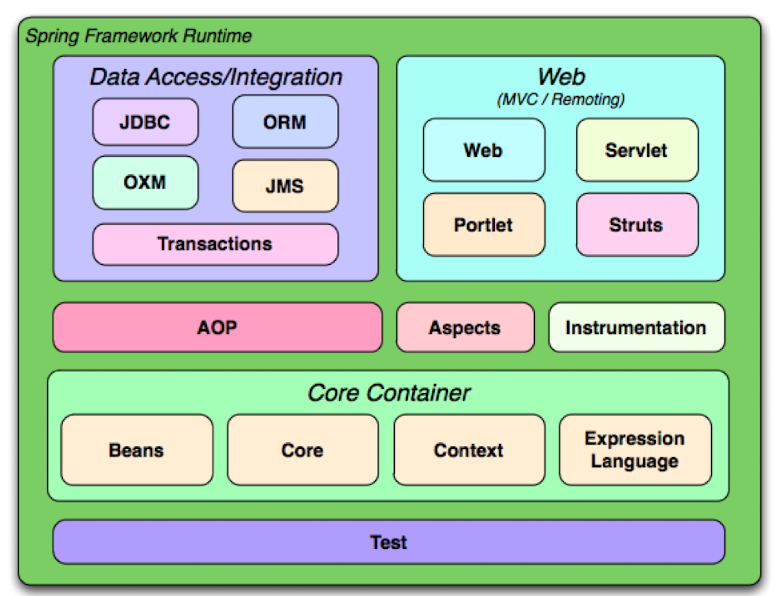
\includegraphics[width=0.75\textwidth]{spring}
  \caption{Spring Framework Overview}
  \label{fig:springframework}
\end{figure}

\subsection{Justification}
Why should we even use a Framework for the development of our software?
\begin{itemize}
	\item To reduce tedious and error prone programming work (create better code)
	\item To raise level of abstraction and convenience by viewpoint/by layer (create less code)
\end{itemize}

Where can and should framework development be considered?
\begin{itemize}
	\item Routine work that has to be done in many place (not domain-specific)
	\item Risky activities such as embedded system development (facing real-time requirements such as guaranteed response time)
	\item Labor-intensive system parts, e.g. user interfaces (server side, client side) and the Web, configuration management and (cloud) deployment
\end{itemize}

\subsection{Spring Annotations}
\begin{table}[H]
  \centering
  \begin{tblr}{colspec={|l|X|},hlines}
    \textbf{Annotation} & \textbf{Meaning} \\
    @SpringBootApplication & Convenience annotation, bundles @Configuration, @EnableAutoConfiguration and @ComponentScan \\
    @Component & The generalized form considered as a candidate for auto-detection when using annotation-based configuration and classpath scanning. It extended to more specific forms such as @Controller, @Repository, and @Service. \\
    @Controller & To indicate C in MVC pattern (presentation layer, dialog control) \\
    @RequestMapping & URI pattern for of RESTful HTTP resources (JEE: JAX-RS) \\
    @Service, @Repository & Specializations of @Component in Spring for DDD (lesson 6) \\
    @Transactional & System transaction (ACID), container is transaction manager \\
    @EnableCaching & Responsible for registering the necessary Spring components that power annotation-driven cache management \\
    @Table, @Entity & Spring Data JPA, steer O/R mapping \\
    @Query & Spring Data JPA, associates query with method \\
    @Profile, @Primary, @Qualifier & Conditional bean registration (OS level, development stage, etc.) \\
    @Autowired & Spring Framework; no need for DI getters/setters (JEE: @Inject) \\
    @JMSListener & Defines the name of the Destination that this method should listen to. (JEE: @MessageDriven) \\
    @JMSTemplate & JmsTemplate class handles the creation and releasing of resources when sending or synchronously receiving messages. (JEE: @Resource) \\

  \end{tblr}
  \caption{Spring Annotations}
\end{table}

\subsection{Spring Concepts}
\begin{description}
  \item [Bean]: A bean is an object that is instantiated, assembled, and otherwise managed by a Spring IoC container. Beans are created with the configuration metadata that you supply to the container. The container then injects those dependencies when it creates the bean. This process is fundamentally the inverse (hence the name, Inversion of Control) of the bean itself controlling the instantiation or location of its dependencies by using direct construction of classes, or a mechanism such as the Service Locator pattern.
  \item [Bean Factory]: The actual container and is responsible for instantiating, configuring, and assembling the beans. The BeanFactory provides an advanced configuration mechanism capable of managing any type of object.
  \item [Application Context]: Is built on top of the BeanFactory and adds more enterprise-specific functionality. It includes all functionality of the BeanFactory and much more. This includes: \textit{a} sophisticated event mechanism for use in a multicaster pattern, \textit{a} resource loading abstraction (for example, to load files from the classpath or the filesystem), \textit{a} hierarchical bean factory capability for managing namespaces, \textit{a} message source for i18n (internationalization), and \textit{a} application-layer specific context such as the WebApplicationContext for use in web applications.
  \item [Spring Boot]: makes it easy to create stand-alone, production-grade Spring based Applications that you can "just run". We take an opinionated view of the Spring platform and third-party libraries so you can get started with minimum fuss. Most Spring Boot applications need very little Spring configuration.
  \item [Service Activator]: A component that receives a message and then delegates to a service to process it.
  \item [Message Channel]: A channel is a conduit that messages can be sent through. Channels are connected to each other, or to message endpoints. Channels can also be connected to message gateways.
  \item [Message Endpoint]: A component that receives messages from a channel.
  \item [Message Gateway]: A component that sends messages to a channel.
  \item [Message Router]: A component that routes a message to one or more channels.
  \item [Data Enricher]: A component that adds data to a message before it is sent to a channel.
\end{description}

\subsection{Inversion of Control}
Inversion of Control is a software design principle, one form of it is Dependency Injection (DI). It is a process whereby objects define their dependencies (that is, the other objects they work with) only through constructor arguments, arguments to a factory method, or properties that are set on the object instance after it is constructed or returned from a factory method.

The Spring Framework uses the Dependency Injection (DI) pattern to manage the components that make up an application. The Spring Framework provides a number of ways to configure a Spring container, including XML, Java \lstinline|@Annotations(...)|.

\subsection{Component Interaction Diagrams (CIDs)}
Component Interaction diagrams describe the dynamic interactions between objects in the system, i.e. pattern of message-passing. This type of diagram can be used additionally in the C4 Model architecture, where it is called Dynamic Diagram, to give a better understanding.

\begin{figure}[H]
  \center
  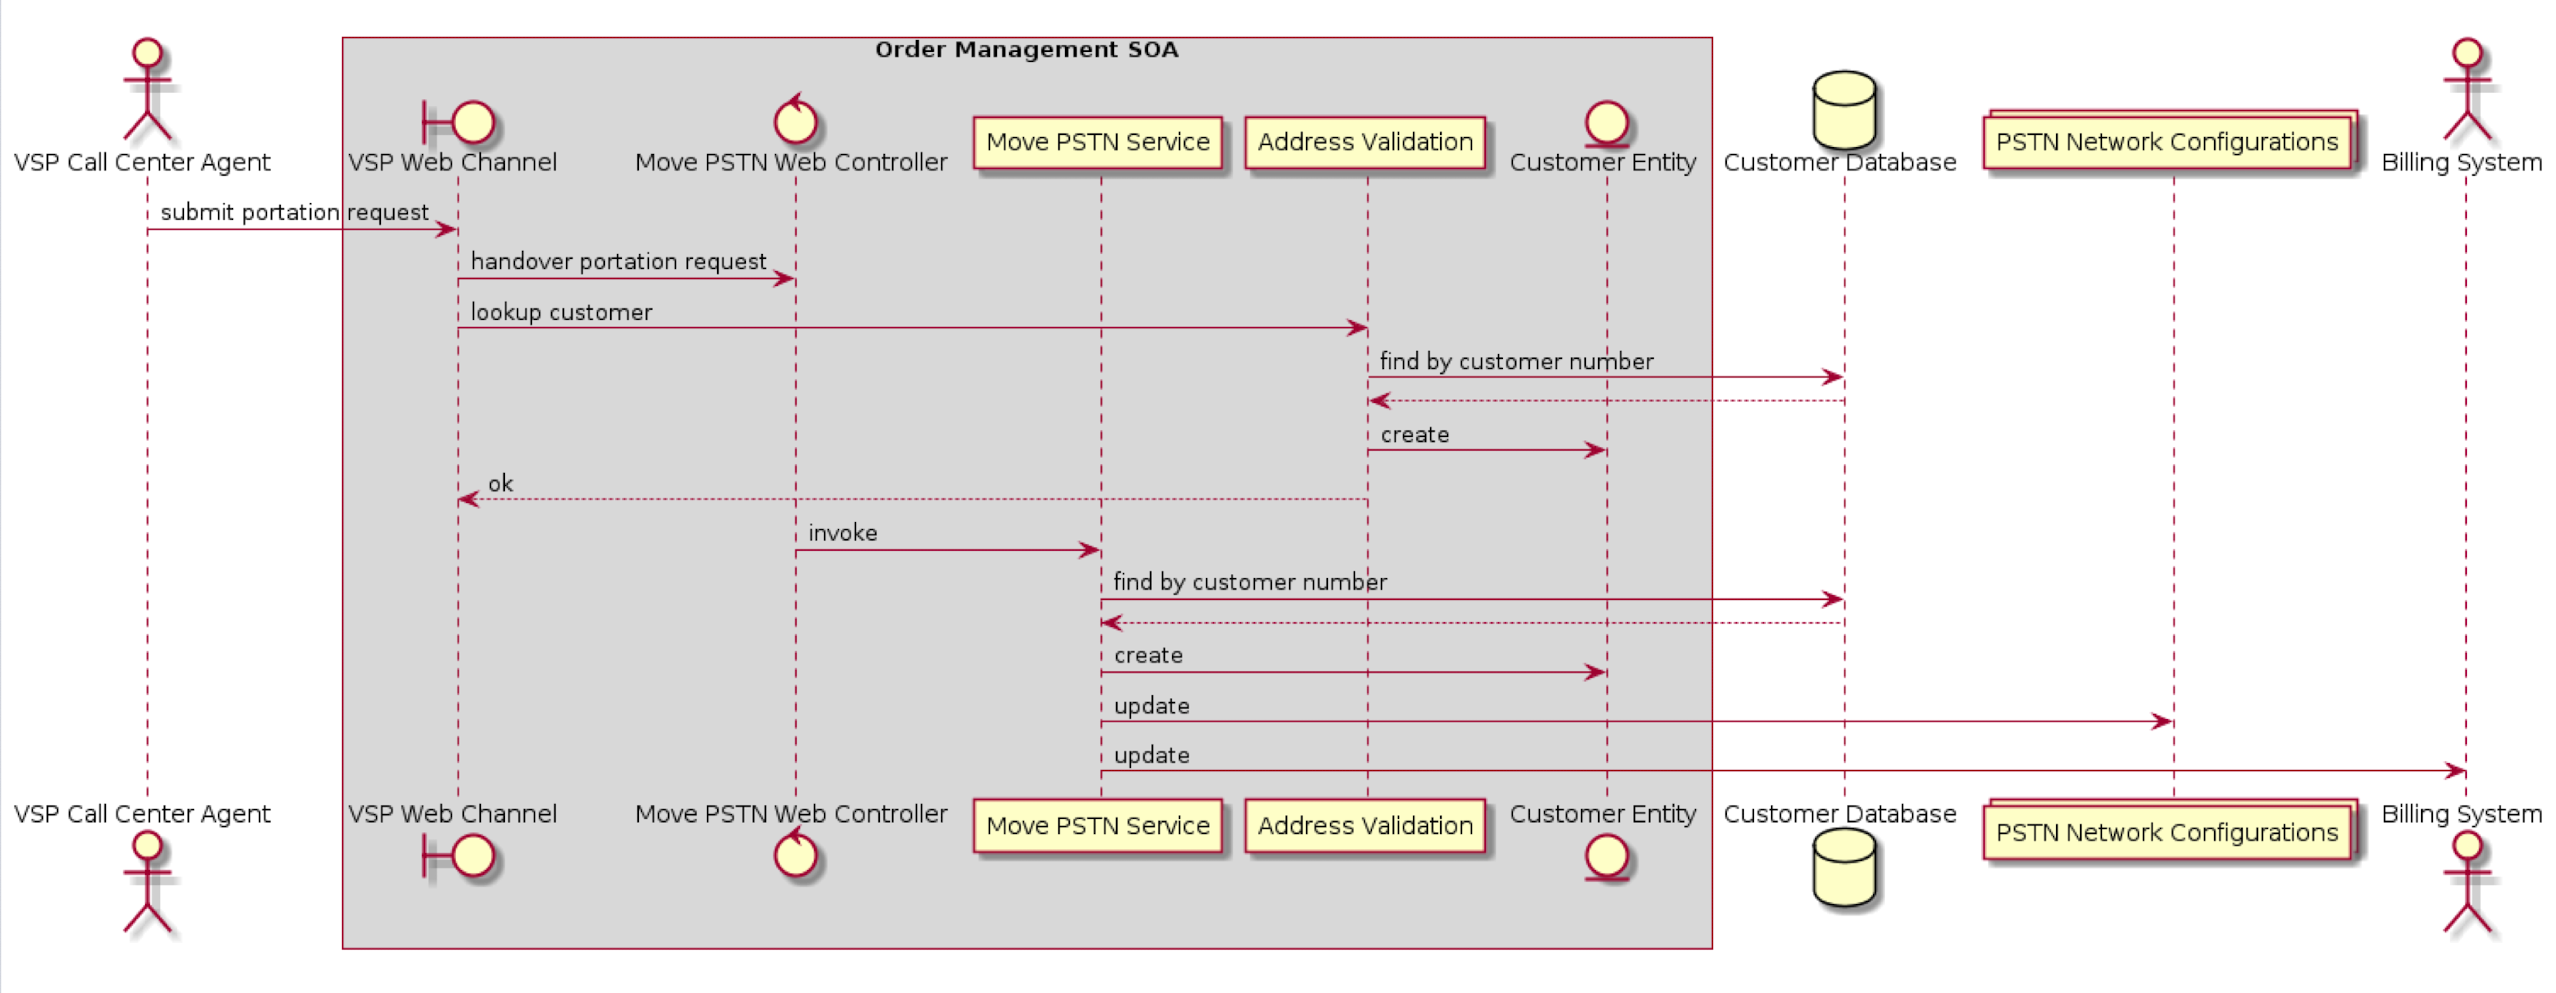
\includegraphics[width=\textwidth]{CIC}
  \caption{Component Interaction Diagram Example}
\end{figure}
